\section{集合代数}
\begin{figure}[htb]
	\def\subwidth{.5\linewidth}
	\centering
	\begin{subfigure}[b]{\subwidth}
		\centering
		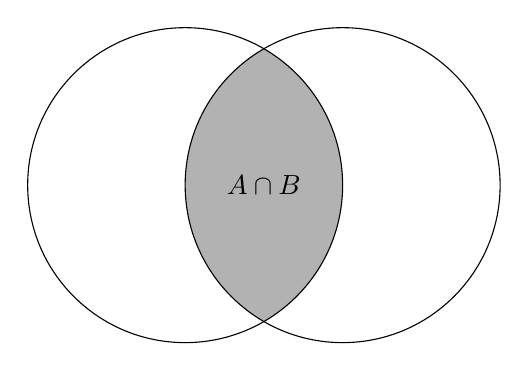
\begin{tikzpicture}
			\path[save path=\pathA](-1,0)circle(2cm);
			\path[save path=\pathB](1,0)circle(2cm);
			\begin{scope}
				\clip[use path=\pathA];
				\fill[black!30][use path=\pathB];
			\end{scope}
			\draw[use path=\pathA];
			\draw[use path=\pathB];
			\draw(0,0)node{\(A \cap B\)};
		\end{tikzpicture}
		\subcaption{集合的交}
	\end{subfigure}%
	\begin{subfigure}[b]{\subwidth}
		\centering
		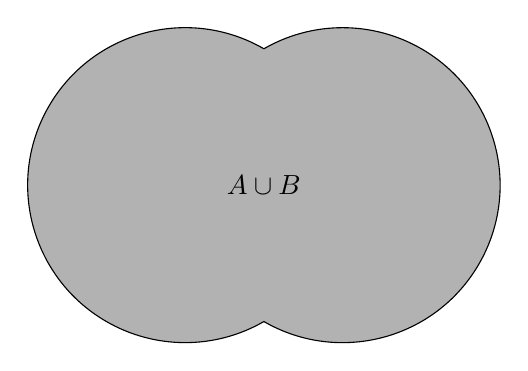
\begin{tikzpicture}
			\filldraw[fill=black!30,draw=black]
				(0,{sqrt(3)})arc[start angle=60,end angle=300,radius=2]
				arc[start angle=240,end angle=480,radius=2];
			\draw(0,0)node{\(A \cup B\)};
			\pgfresetboundingbox
			\path[use as bounding box] (-3,-2)rectangle(3,2);
		\end{tikzpicture}
		\subcaption{集合的并}
	\end{subfigure}%

	\begin{subfigure}[b]{\linewidth}
		\centering
		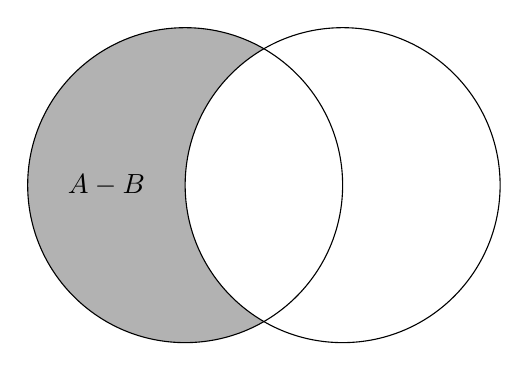
\begin{tikzpicture}
			\fill[black!30](0,{sqrt(3)})arc[start angle=60,end angle=300,radius=2]
				arc[start angle=240,end angle=120,radius=2];
			\draw(-1,0)circle(2cm);
			\draw(1,0)circle(2cm);
			\draw(-2,0)node{\(A-B\)};
			\pgfresetboundingbox
			\path[use as bounding box] (-3,-2)rectangle(3,2);
		\end{tikzpicture}
		\subcaption{集合的差}
	\end{subfigure}%
	\caption{韦恩图}
	\label{figure:集合论.韦恩图}
\end{figure}

\begin{property}
%@see: 《点集拓扑讲义（第四版）》（熊金城） P9 定理1.2.3
集合的运算满足以下性质：
\begin{enumerate}
\item 幂等律
\begin{gather}
	A \cap A = A, \\
	A \cup A = A.
\end{gather}

\item 交换律（{\rm Commutative laws}）
\begin{gather}
	A \cap B = B \cap A, \label{equation:集合论.集合代数公式1-1} \\
	A \cup B = B \cup A, \label{equation:集合论.集合代数公式1-2} \\
	A \symdiff B = B \symdiff A.
\end{gather}

\item 结合律（{\rm Associative laws}）
\begin{gather}
	(A \cap B) \cap C = A \cap (B \cap C), \label{equation:集合论.集合代数公式2-1} \\
	(A \cup B) \cup C = A \cup (B \cup C), \label{equation:集合论.集合代数公式2-2} \\
	%@see: 《测度论讲义（第三版）》（严加安） P4 习题 1.1.1 (1)
	(A \symdiff B) \symdiff C = A \symdiff (B \symdiff C).
\end{gather}

\item 分配律（{\rm Distributive laws}）
\begin{gather}
	(A \cap B) \cup C = (A \cup C) \cap (B \cup C), \label{equation:集合论.集合代数公式3-1} \\
	(A \cup B) \cap C = (A \cap C) \cup (B \cap C), \label{equation:集合论.集合代数公式3-2} \\
	A \cup \bigcap \mathscr{B} = \bigcap\Set{A \cup X \given X \in \mathscr{B}}, \quad(\mathscr{B}\neq\emptyset) \label{equation:集合论.集合代数公式3-3} \\
	A \cap \bigcup \mathscr{B} = \bigcup\Set{A \cap X \given X \in \mathscr{B}}, \label{equation:集合论.集合代数公式3-4} \\
	\Powerset (A \cup B) \supseteq \Powerset A \cup \Powerset B, \label{equation:集合论.集合代数公式3-5} \\ %@see: 《Elements of Set Theory》 P26 Exercise 7(b).
	\Powerset (A \cap B) = \Powerset A \cap \Powerset B, \label{equation:集合论.集合代数公式3-6} \\ %@see: 《Elements of Set Theory》 P26 Exercise 7(a)
	%@see: 《测度论讲义（第三版）》（严加安） P4 习题 1.1.1 (2)
	(A \symdiff B) \cap C = (A \cap C) \symdiff (B \cap C).
\end{gather}

%@see: https://mathworld.wolfram.com/deMorgansLaws.html
\item 对偶律（{\rm De Morgan's laws}）（假设\(\mathscr{A}\neq\emptyset\)）
\begin{gather}
	\Omega - (A \cap B)
	= (\Omega - A) \cup (\Omega - B), \label{equation:集合论.集合代数公式4-1} \\
	\Omega - (A \cup B)
	= (\Omega - A) \cap (\Omega - B), \label{equation:集合论.集合代数公式4-2} \\
	\Omega - \bigcup\mathscr{A}
	= \bigcap\Set{\Omega - X \given X\in\mathscr{A}}, \label{equation:集合论.集合代数公式4-3} \\
	\Omega - \bigcap\mathscr{A}
	= \bigcup\Set{\Omega - X \given X\in\mathscr{A}}. \label{equation:集合论.集合代数公式4-4}
\end{gather}

\item 与空集\(\emptyset\)和全集\(\Omega\)的运算（假设\(A \subseteq \Omega\)）
\begin{gather}
	A \cup \emptyset = A, \label{equation:集合论.集合代数公式5-1} \\
	A \cap \emptyset = \emptyset, \label{equation:集合论.集合代数公式5-2} \\
	A \cup \Omega = \Omega, \label{equation:集合论.集合代数公式5-3} \\
	A \cap \Omega = A, \label{equation:集合论.集合代数公式5-4} \\
	A \cup (\Omega - A) = \Omega, \label{equation:集合论.集合代数公式5-5} \\
	A \cap (\Omega - A) = \emptyset, \label{equation:集合论.集合代数公式5-6} \\
	A \cup (A \cap B) = A, \\
	A \cap (A \cup B) = A, \\
	\Omega - \emptyset = \Omega, \\
	\Omega - \Omega = \emptyset, \\
	%@see: 《点集拓扑讲义（第四版）》（熊金城） P10 习题 1.(3)
	\Omega - (\Omega - A) = A.
\end{gather}

\item 包含关系
\begin{gather}
	%@see: 《点集拓扑讲义（第四版）》（熊金城） P10 习题 1.(2)
	A \subseteq B \implies A \cup C \subseteq B \cup C, \label{equation:集合论.集合代数公式6-1} \\
	%@see: 《点集拓扑讲义（第四版）》（熊金城） P10 习题 1.(2)
	A \subseteq B \implies A \cap C \subseteq B \cap C, \label{equation:集合论.集合代数公式6-2} \\
	A \subseteq B \implies \bigcup A \subseteq \bigcup B, \label{equation:集合论.集合代数公式6-3} \\
	A \subseteq B \subseteq \Omega \implies (\Omega - B) \subseteq (\Omega - A), \label{equation:集合论.集合代数公式6-4} \\
	\emptyset \neq A \subseteq B \implies \bigcap B \subseteq \bigcap A, \label{equation:集合论.集合代数公式6-5} \\
	%@see: 《点集拓扑讲义（第四版）》（熊金城） P10 习题 1.(1)
	A \cap B \subseteq A, \\
	%@see: 《点集拓扑讲义（第四版）》（熊金城） P10 习题 1.(1)
	A \subseteq A \cup B, \label{equation:集合论.集合代数公式6-7} \\
	(A \subseteq C) \land (B \subseteq C) \iff A \cup B \subseteq C, \label{equation:集合论.集合代数公式6-8} \\
	(A \subseteq B) \land (A \subseteq C) \iff A \subseteq B \cap C, \label{equation:集合论.集合代数公式6-9} \\
	%@see: 《测度论讲义（第三版）》（严加安） P4 习题 1.1.1 (3)
	(A \cup B) \symdiff (C \cup D) \subseteq (A \symdiff C) \cup (B \symdiff D).
\end{gather}

\item 差集和对称差
\begin{gather}
	A - A = \emptyset, \\
	A - B \subseteq A, \\
	%@see: 《点集拓扑讲义（第四版）》（熊金城） P10 习题 2.(1)
	A \subseteq \Omega
	\implies
	A - B = A \cap (\Omega - B), \\
	A \cup B = B
		\iff A \subseteq B
		\iff A \cap B = A
		\iff A - B = \emptyset, \label{equation:集合论.集合代数公式7-3} \\
	A \symdiff \emptyset = A, \\
	A \symdiff A = \emptyset, \\
	A \symdiff B = A \symdiff C
		\iff B = C.
\end{gather}
\end{enumerate}
    \begin{proof}
        任取元素\(x\).
        在各段证明中，
        用\(p,q,r,s,w\)依次表示命题\(x\in A,x\in B,x\in C,x\in D,x\in\Omega\).
        由集合运算的定义及异或联结词的真值表，
        有
        \begin{align*}
            x\in A\cap B &\iff p\land q, \\
            x\in A\cup B &\iff p\lor q, \\
            x\in A-B &\iff p\land\neg q, \\
            x\in A\symdiff B &\iff (p\land\neg q)\lor(q\land\neg p)
            \iff p\lxor q.
        \end{align*}
        以下使用\cref{theorem:数理逻辑.基本等值式}及命题逻辑中异或的交换律、结合律进行等值演算.
        对于任意\(x\)都成立的成员资格等价式，
        由外延公理给出集合相等；成员资格的蕴含式，
        则由\cref{definition:集合论.子集的定义}给出包含关系.
        涉及集族时，
        还使用量词的语义及下列成员资格判定：
        \begin{align*}
            x\in\bigcup\mathscr{F}
            &\iff (\exists X)[X\in\mathscr{F}\land x\in X], \\
            x\in\bigcap\mathscr{F}
            &\iff (\forall X)[X\in\mathscr{F}\limp x\in X],
            \quad\mathscr{F}\neq\emptyset.
        \end{align*}
        后一式的非空条件来自\cref{theorem:集合论.系的交的唯一存在性}.
        本节不对\(\bigcap\emptyset\)另作约定.
        \begin{enumerate}
            \item 幂等律.
            \begin{align*}
                x\in A\cap A
                &\iff p\land p\iff p\iff x\in A, \tag{合取幂等律}\\
                x\in A\cup A
                &\iff p\lor p\iff p\iff x\in A. \tag{析取幂等律}
            \end{align*}

            \item 交换律.
            \begin{align*}
                x\in A\cap B
                &\iff p\land q\iff q\land p\iff x\in B\cap A, \tag{合取交换律}\\
                x\in A\cup B
                &\iff p\lor q\iff q\lor p\iff x\in B\cup A, \tag{析取交换律}\\
                x\in A\symdiff B
                &\iff p\lxor q\iff q\lxor p\iff x\in B\symdiff A. \tag{异或交换律}
            \end{align*}

            \item 结合律.
            \begin{align*}
                x\in(A\cap B)\cap C
                &\iff(p\land q)\land r \\
                &\iff p\land(q\land r) \tag{合取结合律}\\
                &\iff x\in A\cap(B\cap C), \\
                x\in(A\cup B)\cup C
                &\iff(p\lor q)\lor r \\
                &\iff p\lor(q\lor r) \tag{析取结合律}\\
                &\iff x\in A\cup(B\cup C), \\
                x\in(A\symdiff B)\symdiff C
                &\iff(p\lxor q)\lxor r \\
                &\iff p\lxor(q\lxor r) \tag{异或结合律}\\
                &\iff x\in A\symdiff(B\symdiff C).
            \end{align*}

            \item 分配律.
            对于前两个分配式，
            有
            \begin{align*}
                x\in(A\cap B)\cup C
                &\iff(p\land q)\lor r \\
                &\iff(p\lor r)\land(q\lor r) \tag{分配律、交换律}\\
                &\iff x\in(A\cup C)\cap(B\cup C), \\
                x\in(A\cup B)\cap C
                &\iff(p\lor q)\land r \\
                &\iff(p\land r)\lor(q\land r) \tag{分配律、交换律}\\
                &\iff x\in(A\cap C)\cup(B\cap C).
            \end{align*}

            设\(\mathscr{B}\neq\emptyset\).
            因为命题\(p\)不含变元\(X\)，
            有
            \begin{align*}
                x\in A\cup\bigcap\mathscr{B}
                &\iff p\lor(\forall X\in\mathscr{B})[x\in X] \\
                &\iff(\forall X\in\mathscr{B})[p\lor x\in X] \tag{全称量词与析取}\\
                &\iff(\forall X\in\mathscr{B})[x\in A\cup X] \\
                &\iff x\in\bigcap\Set{A\cup X\given X\in\mathscr{B}}.
            \end{align*}
            上述量词变换可以按\(p\)的真值验证：当\(p\)为真时两边均真，
            当\(p\)为假时两边均化为\((\forall X\in\mathscr{B})[x\in X]\).
            \(\mathscr{B}\)非空还保证右端被取交的集族非空.

            对于任意集族\(\mathscr{B}\)，
            有
            \begin{align*}
                x\in A\cap\bigcup\mathscr{B}
                &\iff p\land(\exists X\in\mathscr{B})[x\in X] \\
                &\iff(\exists X\in\mathscr{B})[p\land x\in X] \tag{存在量词与合取}\\
                &\iff(\exists X\in\mathscr{B})[x\in A\cap X] \\
                &\iff x\in\bigcup\Set{A\cap X\given X\in\mathscr{B}}.
            \end{align*}
            这里两边使用同一个存在量词的见证\(X\)；若\(\mathscr{B}=\emptyset\)，
            则两边的存在命题均为假，
            相应集合均为空集.

            对于\cref{equation:集合论.集合代数公式3-5}，
            任取集合\(Y\)，
            有
            \begin{align*}
                Y\in\Powerset A\cup\Powerset B
                &\iff(Y\subseteq A)\lor(Y\subseteq B) \tag{并集、幂集的定义}\\
                &\implies Y\subseteq A\cup B \tag{子集的定义}\\
                &\iff Y\in\Powerset(A\cup B).
            \end{align*}
            中间的蕴含不能普遍改成等价.
            例如取\(A=\Set{1},B=\Set{2},Y=\Set{1,2}\)，
            则
            \begin{align*}
                Y&\subseteq A\cup B, \\
                Y&\not\subseteq A, \\
                Y&\not\subseteq B.
            \end{align*}
            因此该例中的包含关系是严格的.

            对于\cref{equation:集合论.集合代数公式3-6}，
            任取集合\(Y\)，
            有
            \begin{align*}
                Y\in\Powerset(A\cap B)
                &\iff(\forall y\in Y)[y\in A\land y\in B] \tag{幂集、交集的定义}\\
                &\iff(\forall y\in Y)[y\in A]\land(\forall y\in Y)[y\in B]
                \tag{全称量词与合取}\\
                &\iff(Y\subseteq A)\land(Y\subseteq B) \\
                &\iff Y\in\Powerset A\cap\Powerset B.
            \end{align*}

            最后证明交对对称差的分配律.
            当\(r\)为假时，
            \((p\lxor q)\land r\)与\((p\land r)\lxor(q\land r)\)均为假；当\(r\)为真时，
            两者均化为\(p\lxor q\).
            故
            \begin{align*}
                x\in(A\symdiff B)\cap C
                &\iff(p\lxor q)\land r \\
                &\iff(p\land r)\lxor(q\land r) \tag{按合取因子分类}\\
                &\iff x\in(A\cap C)\symdiff(B\cap C).
            \end{align*}

            \item 对偶律.
            不必假设\(A,B\)是\(\Omega\)的子集，
            直接有
            \begin{align*}
                x\in\Omega-(A\cap B)
                &\iff w\land\neg(p\land q) \\
                &\iff w\land(\neg p\lor\neg q) \tag{德摩根律}\\
                &\iff(w\land\neg p)\lor(w\land\neg q) \tag{合取分配律}\\
                &\iff x\in(\Omega-A)\cup(\Omega-B), \\
                x\in\Omega-(A\cup B)
                &\iff w\land\neg(p\lor q) \\
                &\iff w\land(\neg p\land\neg q) \tag{德摩根律}\\
                &\iff(w\land\neg p)\land(w\land\neg q) \tag{结合律、幂等律}\\
                &\iff x\in(\Omega-A)\cap(\Omega-B).
            \end{align*}

            设\(\mathscr{A}\neq\emptyset\).
            由量词否定规则得
            \begin{align*}
                x\in\Omega-\bigcup\mathscr{A}
                &\iff w\land\neg(\exists X\in\mathscr{A})[x\in X] \\
                &\iff w\land(\forall X\in\mathscr{A})[x\notin X] \tag{否定存在量词}\\
                &\iff(\forall X\in\mathscr{A})[w\land x\notin X] \tag{集族非空}\\
                &\iff(\forall X\in\mathscr{A})[x\in\Omega-X] \\
                &\iff x\in\bigcap\Set{\Omega-X\given X\in\mathscr{A}}, \\
                x\in\Omega-\bigcap\mathscr{A}
                &\iff w\land\neg(\forall X\in\mathscr{A})[x\in X] \\
                &\iff w\land(\exists X\in\mathscr{A})[x\notin X] \tag{否定全称量词}\\
                &\iff(\exists X\in\mathscr{A})[w\land x\notin X] \tag{存在量词与合取}\\
                &\iff(\exists X\in\mathscr{A})[x\in\Omega-X] \\
                &\iff x\in\bigcup\Set{\Omega-X\given X\in\mathscr{A}}.
            \end{align*}
            第一串等价式中，
            从全称命题取出\(w\)需要\(\mathscr{A}\neq\emptyset\)：取\(X_0\in\mathscr{A}\)，
            即可由\(w\land x\notin X_0\)推出\(w\).
            此外，
            非空条件保证两条公式涉及的交集都有定义.

            \item 与空集和全集的运算.
            由\(A\subseteq\Omega\)，
            知\(p\limp w\)为真，
            所以\(p\lor w\)等值于\(w\)，
            \(p\land w\)等值于\(p\).
            结合基本等值式，
            逐一得到
            \begin{align*}
                x\in A\cup\emptyset
                &\iff p\lor0\iff p\iff x\in A, \tag{同一律}\\
                x\in A\cap\emptyset
                &\iff p\land0\iff0\iff x\in\emptyset, \tag{0-1律}\\
                x\in A\cup\Omega
                &\iff p\lor w\iff w\iff x\in\Omega, \tag{包含关系}\\
                x\in A\cap\Omega
                &\iff p\land w\iff p\iff x\in A, \tag{包含关系}\\
                x\in A\cup(\Omega-A)
                &\iff p\lor(w\land\neg p) \\
                &\iff(p\lor w)\land(p\lor\neg p) \tag{析取分配律}\\
                &\iff w\land1\iff w\iff x\in\Omega, \tag{包含关系、互补律}\\
                x\in A\cap(\Omega-A)
                &\iff p\land w\land\neg p\iff0\iff x\in\emptyset, \tag{互补律}\\
                x\in A\cup(A\cap B)
                &\iff p\lor(p\land q)\iff p\iff x\in A, \tag{吸收律}\\
                x\in A\cap(A\cup B)
                &\iff p\land(p\lor q)\iff p\iff x\in A, \tag{吸收律}\\
                x\in\Omega-\emptyset
                &\iff w\land\neg0\iff w\iff x\in\Omega, \tag{同一律}\\
                x\in\Omega-\Omega
                &\iff w\land\neg w\iff0\iff x\in\emptyset, \tag{互补律}\\
                x\in\Omega-(\Omega-A)
                &\iff w\land\neg(w\land\neg p) \\
                &\iff w\land(\neg w\lor p) \tag{德摩根律、对合律}\\
                &\iff(w\land\neg w)\lor(w\land p) \tag{合取分配律}\\
                &\iff p\iff x\in A. \tag{互补律、包含关系}
            \end{align*}

            \item 包含关系.
            先设\(A\subseteq B\)，
            则对任意\(x\)都有\(p\limp q\).
            由分类讨论及合取的语义，
            有
            \begin{align*}
                x\in A\cup C
                &\iff p\lor r\implies q\lor r\iff x\in B\cup C, \\
                x\in A\cap C
                &\iff p\land r\implies q\land r\iff x\in B\cap C.
            \end{align*}
            这分别给出\cref{equation:集合论.集合代数公式6-1,equation:集合论.集合代数公式6-2}.
            同一假设下，
            并集中的见证也可以保留，
            所以
            \begin{align*}
                x\in\bigcup A
                &\iff(\exists T)[T\in A\land x\in T] \\
                &\implies(\exists T)[T\in B\land x\in T] \tag{包含关系}\\
                &\iff x\in\bigcup B.
            \end{align*}

            若\(A\subseteq B\subseteq\Omega\)，
            由\(p\limp q\)的逆否命题\(\neg q\limp\neg p\)，
            得
            \begin{align*}
                x\in\Omega-B
                &\iff w\land\neg q \\
                &\implies w\land\neg p \tag{逆否命题}\\
                &\iff x\in\Omega-A.
            \end{align*}

            若\(\emptyset\neq A\subseteq B\)，
            则\(B\neq\emptyset\)，
            两个交集都有定义，
            且
            \begin{align*}
                x\in\bigcap B
                &\iff(\forall T\in B)[x\in T] \\
                &\implies(\forall T\in A)[x\in T] \tag{缩小全称量词的范围}\\
                &\iff x\in\bigcap A.
            \end{align*}

            不附加条件时，
            由合取的化简及析取的附加可得
            \begin{align*}
                x\in A\cap B
                &\iff p\land q\implies p\iff x\in A, \\
                x\in A
                &\iff p\implies p\lor q\iff x\in A\cup B.
            \end{align*}

            对\cref{equation:集合论.集合代数公式6-8}，
            将子集关系展开为全称命题，
            得到
            \begin{align*}
                (A\subseteq C)\land(B\subseteq C)
                &\iff(\forall x)[(x\in A\limp x\in C)\land(x\in B\limp x\in C)] \\
                &\iff(\forall x)[(x\in A\lor x\in B)\limp x\in C]
                \tag{蕴含化为析取、分配律}\\
                &\iff A\cup B\subseteq C.
            \end{align*}
            第一步使用了全称量词对合取的分配：两条命题对每个\(x\)分别成立，
            当且仅当它们的合取对每个\(x\)成立.
            同理，
            对于\cref{equation:集合论.集合代数公式6-9}，
            有
            \begin{align*}
                (A\subseteq B)\land(A\subseteq C)
                &\iff(\forall x)[(x\in A\limp x\in B)\land(x\in A\limp x\in C)] \\
                &\iff(\forall x)[x\in A\limp(x\in B\land x\in C)]
                \tag{蕴含化为析取、分配律}\\
                &\iff A\subseteq B\cap C.
            \end{align*}

            最后一个对称差包含式用逆否命题证明.
            若\(x\notin(A\symdiff C)\cup(B\symdiff D)\)，
            则
            \begin{align*}
                x\notin(A\symdiff C)\cup(B\symdiff D)
                &\iff\neg(p\lxor r)\land\neg(q\lxor s) \tag{德摩根律}\\
                &\iff(p\liff r)\land(q\liff s) \tag{异或与等价的关系}\\
                &\implies(p\lor q)\liff(r\lor s) \tag{析取的真值}\\
                &\iff\neg\bigl((p\lor q)\lxor(r\lor s)\bigr) \\
                &\iff x\notin(A\cup B)\symdiff(C\cup D).
            \end{align*}
            取逆否命题，
            便得到所需包含关系.

            \item 差集.
            首先有
            \begin{align*}
                x\in A-A
                &\iff p\land\neg p\iff0\iff x\in\emptyset, \tag{互补律}\\
                x\in A-B
                &\iff p\land\neg q\implies p\iff x\in A. \tag{合取的化简}
            \end{align*}

            对于差集与相对补集的关系，
            所用条件是\(A\subseteq\Omega\)，
            而不是仅有\(B\subseteq\Omega\).
            此时\(p\limp w\)，
            所以
            \begin{align*}
                x\in A-B
                &\iff p\land\neg q \\
                &\iff p\land w\land\neg q \tag{包含关系}\\
                &\iff x\in A\cap(\Omega-B).
            \end{align*}
            原条件不足的反例是\(A=\Set{1},B=\Omega=\emptyset\)：虽然\(B\subseteq\Omega\)，
            却有
            \begin{align*}
                A-B&=\Set{1}, \\
                A\cap(\Omega-B)&=\emptyset.
            \end{align*}

            对\cref{equation:集合论.集合代数公式7-3}，
            分别把三个等式化为同一全称命题：
            \begin{align*}
                A\cup B=B
                &\iff(\forall x)[(x\in A\lor x\in B)\liff x\in B] \\
                &\iff(\forall x)[x\in A\limp x\in B] \tag{蕴含、等价的真值}\\
                &\iff A\subseteq B, \\
                A\cap B=A
                &\iff(\forall x)[(x\in A\land x\in B)\liff x\in A] \\
                &\iff(\forall x)[x\in A\limp x\in B] \tag{蕴含、等价的真值}\\
                &\iff A\subseteq B, \\
                A-B=\emptyset
                &\iff\neg(\exists x)[x\in A\land x\notin B] \\
                &\iff(\forall x)[\neg(x\in A\land x\notin B)] \tag{否定存在量词}\\
                &\iff(\forall x)[x\in A\limp x\in B] \tag{德摩根律、蕴含等值式}\\
                &\iff A\subseteq B.
            \end{align*}
            这证明了原式中的全部等价关系.

            由异或的真值表，
            又有
            \begin{align*}
                x\in A\symdiff\emptyset
                &\iff p\lxor0\iff p\iff x\in A, \\
                x\in A\symdiff A
                &\iff p\lxor p\iff0\iff x\in\emptyset.
            \end{align*}
            若\(A\symdiff B=A\symdiff C\)，
            则利用已经证明的对称差交换律、结合律及上面两式，
            得到
            \begin{align*}
                B&=(A\symdiff A)\symdiff B \tag{同集对称差、空集运算}\\
                &=A\symdiff(A\symdiff B) \tag{结合律}\\
                &=A\symdiff(A\symdiff C) \tag{已知条件}\\
                &=(A\symdiff A)\symdiff C \tag{结合律}\\
                &=C. \tag{同集对称差、空集运算}
            \end{align*}
            反过来，
            若\(B=C\)，
            则由相等对象的替换立即得到\(A\symdiff B=A\symdiff C\).
        \end{enumerate}
    \end{proof}
\end{property}

\begin{example}
    %@see: 《Elements of Set Theory》 P32 Exercise 21.
    设\(A,B\)是集合.
    证明：\begin{equation}\label{equation:集合论.并集的并等于并的并集}
        \bigcup(A\cup B)=\bigcup A\cup\bigcup B.
    \end{equation}
    \begin{proof}
        任取\(x\)，
        由并集的定义有
        \begin{align*}
            x\in\bigcup(A\cup B)
            &\iff(\exists T)[T\in A\cup B\land x\in T] \\
            &\iff(\exists T)[(T\in A\lor T\in B)\land x\in T] \\
            &\iff(\exists T)[(T\in A\land x\in T)\lor(T\in B\land x\in T)]
            \tag{合取分配律}\\
            &\iff(\exists T\in A)[x\in T]\lor(\exists T\in B)[x\in T]
            \tag{存在量词与析取}\\
            &\iff x\in\bigcup A\cup\bigcup B.
        \end{align*}
        存在量词中的成员条件必须与\(x\in T\)合取，
        不能写成蕴含：不属于集族的\(T\)不能作为并集成员资格的见证.
        由\(x\)的任意性和外延公理得证.
    \end{proof}
\end{example}

\begin{example}
    %@see: 《Elements of Set Theory》 P32 Exercise 22.
    设\(A,B\)是非空集合.
    证明：\begin{equation}
        \bigcap(A\cup B)=\bigcap A\cap\bigcap B.
    \end{equation}
    \begin{proof}
        由于\(A,B\)均非空，
        \(A\cup B\)也非空，
        所以三个集族的交都有定义.
        任取\(x\)，
        有
        \begin{align*}
            x\in\bigcap(A\cup B)
            &\iff(\forall T)[T\in A\cup B\limp x\in T] \\
            &\iff(\forall T)[(T\in A\lor T\in B)\limp x\in T] \\
            &\iff(\forall T)[(T\in A\limp x\in T)\land(T\in B\limp x\in T)]
            \tag{蕴含化为析取、分配律}\\
            &\iff(\forall T\in A)[x\in T]\land(\forall T\in B)[x\in T]
            \tag{全称量词与合取}\\
            &\iff x\in\bigcap A\cap\bigcap B.
        \end{align*}
        由外延公理得证.
    \end{proof}
\end{example}

\begin{example}
    证明：\begin{equation}
        (A\cup B)-(A\cap B)=(A-B)\cup(B-A).
    \end{equation}
    \begin{proof}
        任取\(x\)，
        用\(p,q\)分别表示命题\(x\in A,x\in B\).
        根据交、并、差的定义及基本等值式，
        有
        \begin{align*}
            x\in(A\cup B)-(A\cap B)
            &\iff(p\lor q)\land\neg(p\land q) \\
            &\iff(p\lor q)\land(\neg p\lor\neg q) \tag{德摩根律}\\
            &\iff\bigl(p\land(\neg p\lor\neg q)\bigr)
            \lor\bigl(q\land(\neg p\lor\neg q)\bigr) \tag{合取分配律}\\
            &\iff\bigl((p\land\neg p)\lor(p\land\neg q)\bigr)
            \lor\bigl((q\land\neg p)\lor(q\land\neg q)\bigr) \tag{合取分配律}\\
            &\iff(p\land\neg q)\lor(q\land\neg p) \tag{互补律、同一律}\\
            &\iff x\in(A-B)\cup(B-A).
        \end{align*}
        由外延公理得证.
    \end{proof}
\end{example}
